\documentclass[paper=a4, fontsize=11pt]{scrartcl}
\usepackage{titling}
\usepackage{dirtytalk}
\usepackage{mathtools}
\usepackage{multirow}
\DeclarePairedDelimiter{\ceil}{\lceil}{\rceil}
    
    \date{}
    \setlength{\droptitle}{-10em}
    \title{\textbf{Raport tema nr 1}}

\begin{document}

\maketitle
\vspace{-7em}
\section{Descrierea problemei}
\paragraph{}
Să se determine minimul pentru următoarele funcții: De Jong 1, Schwefel 7, Rastrigin, Six-hump camel back implementând algoritmii Hill Climbing (variantele First Improvement și Best Improvement) și Simulated Annealing. 

\section{Algoritmul utilizat}
\paragraph{}
Ideea algoritmului constă în faptul că, pentru o soluție curentă $x=(x_1,...x_n)$, vecinii acestei soluții pot conduce la soluții mai bune. Deci evaluăm funcția în vecinii soluției curente, folosind algoritmii Hill Climbing și Simulated Annealing.
\subparagraph{2.1}
\textbf{Hill Climbing}, pseudocod:

\begin{itemize}
    \item[] Pentru Best Improvement:
    \begin{itemize}
        \item[] Cât timp (mai există iterații de făcut)
        \begin{enumerate}
            \item Generează o soluție random și evaluează funcția pentru această soluție.
            \item Generează vecinii acestei soluții.
            \item Evaluează funcția pentru fiecare vecin.
            \item Selectează cel mai bun vecin - bestNeighbour.
            \item Dacă bestNeighbour este mai bun decât soluția curentă, soluția curentă devine bestNeighbour, și sare la punctul 2. Altfel, trece la următoarea iterație.
            \item Returnează cea mai bună soluție.
        \end{enumerate} 
    \end{itemize}
    \item[] Pentru First Improvement: 
    \begin{itemize}
        \item[] În loc să selecteze cel mai bun vecin, algoritmul selectează primul vecin care îmbunătățește soluția, chiar dacă nu este cel mai bun.
    \end{itemize} 
\end{itemize}

\textbf{Simulated Annealing}, pseudocod:

\begin{itemize}
    \item[] Cât timp (mai există iterații de făcut)
    \begin{enumerate}
        \item Generează o soluție random și evaluează funcția pentru această soluție.
        \item Cât timp (nu s-a ajuns la o răcire absolută)
        \begin{enumerate}
            \item Generează vecinii soluției curente și selectează un vecin random.
            \item Evaluează funcția pentru acel vecin - neighbourValue.
            \item Soluția curentă devine neighbourValue dacă neighbourValue este mai bun sau dacă temperatura curentă permite selectarea lui, chiar dacă nu este mai bun, și sare la punctul 2. Altfel, sare la punctul 1 (la următoarea iterație).
            \item Temperatura se răcește.
        \end{enumerate}
        \item Returnează cea mai bună soluție.
    \end{enumerate}
\end{itemize} 

\subparagraph{2.1}
Detalii de implementare

\paragraph{}
\underline{\smash{Reprezentarea soluțiilor}} a fost făcută pe șiruri binare, astfel: 
\say{Spaţiul de căutare se va disctretiza până la o anumită precizie $10^{-d}$. 
Un interval [a, b] va fi împărţit în N = $(b-a)*(10^d)$ subintervale egale.
Pentru a putea reprezenta cele $(b-a)*(10^d)$ valori, este nevoie de un număr n = $\ceil{log_2N}$ de biţi.
Lungimea şirului de biţi care reprezintă o soluţie candidat va fi suma lungimilor reprezentărilor pentru fiecare parametru al funcţiei de optimizat. În momentul evaluării soluției (apelul funcției de optimizat) este necesară decodificarea fiecărui parametru reprezentat ca șir de biți în număr real, după formula: $X_{real} = a + decimal(x_{biti})*(b-a)/(2^n-1)$.}

\underline{\smash{Vecinii}} sunt construiți prin schimbarea câte unui bit, pe rând, în reprezentarea binară a soluției.

\underline{\smash{Inițializarea}} constă în crearea random a unei soluții binare. 

Pentru Hill Climbing, \underline{\smash{condiția de oprire}} este negăsirea niciunui vecin care să îmbunătățească soluția curentă, semn că am ajuns la un minim. Pentru Simulated Annealing, pe lângă condiția de oprire de la Hill Climbing, mai avem și condiția ca temperatura să nu fi ajuns la o valoare foarte mică.

În funcție de punctul de plecare al temperaturii și de funcția de răcire, algoritmul Simulated Annealing se comportă foarte asemănător cu Hill Climbing, deoarece, dacă temperatura aleasă este foarte mică, șansa ca o soluție mai proastă să treacă mai departe este mult mai mică, iar Hill Climbing nu alege niciodată soluții proaste; astfel cele două metode sunt asemănătoare.

\section{Rezultate experimentale}

\begin{table}[h]
    \resizebox{1.15\textwidth}{!}{\begin{tabular}{|l|l|l|l|l|l|l|l|l|l|l|l|l|}
    \hline
    \multicolumn{2}{|c|}{Algoritm}                 & \multicolumn{1}{|c|}{Funcție}                                              & Dimensiuni & Rulări                  & Minim    & Medie   & Maxim  & Deviație          & Minim   & Medie    & Maxim   & Deviație       \\ \hline
    \multicolumn{5}{|l|}{}                                                                                                                                             & \multicolumn{4}{|c|}{Best Improvement}          & \multicolumn{4}{|c|}{First Improvement}       \\ \hline
    \multicolumn{2}{|l|}{\multirow{12}{*}{\begin{tabular}[c]{@{}l@{}}Hill\\ Climbing\end{tabular}}} & \multirow{3}{*}{De Jong}  & 5          & \multirow{3}{*}{30}     & 1.204    & 4.647   & 9.574  & 4.966             & 1.137    & 4.296   & 8.205   & 5.987          \\
    \multicolumn{2}{|l|}{}                          &                                                                           & 10         &                         & 10.44    & 23.24   & 34.67  & 12.28             & 14.69    & 25.40   & 41.40   & 9.950          \\ 
    \multicolumn{2}{|l|}{}                          &                                                                           & 30         &                         & 98.07    & 145.3   & 168.8  & 20.53             & 134.2    & 149.7   & 169.2   & 8.969          \\ \cline{3-13} 
    \multicolumn{2}{|l|}{}                          & \multirow{3}{*}{Rastrigin}                                                & 5          & \multirow{3}{*}{30}     & 14.21    & 30.57   & 43.29  & 18.54             & 14.21    & 30.20   & 39.74   & 14.49          \\  
    \multicolumn{2}{|l|}{}                          &                                                                           & 10         &                         & 68.71    & 93.05   & 114.2  & 18.50             & 66.86    & 96.10   & 116.2   & 21.05          \\  
    \multicolumn{2}{|l|}{}                          &                                                                           & 30         &                         & 337.5    & 390.8   & 423.1  & 24.60             & 335.9    & 392.3   & 417.1   & 18.74          \\ \cline{3-13} 
    \multicolumn{2}{|l|}{}                          & \multirow{3}{*}{Schwefel 7}                                               & 5          & \multirow{3}{*}{30}     & -1801    & -1260   & 0      & 505               & -1810    & -1188   & 0       & 457.5          \\  
    \multicolumn{2}{|l|}{}                          &                                                                           & 10         &                         & -2128    & -1871   & 0      & 186.8             & -2714    & -1909   & 0       & 329.6          \\ 
    \multicolumn{2}{|l|}{}                          &                                                                           & 30         &                         & -5525    & -5489   & 0      & 51.47             & -5529    & -5499   & 0       & 38.92          \\ \cline{3-13} 
    \multicolumn{2}{|l|}{}                          & \multirow{3}{*}{\begin{tabular}[c]{@{}l@{}}Six-hump\\ camel back\end{tabular}} & \multirow{3}{*}{2}              & \multirow{3}{*}{30}     & \multirow{3}{*}{-1.02}        & \multirow{3}{*}{-0.95}        & \multirow{3}{*}{0}       & \multirow{3}{*}{0.38}          & \multirow{3}{*}{-1.03}         & \multirow{3}{*}{-0.96}       & \multirow{3}{*}{0}       & \multirow{3}{*}{0.235}          \\ 
    \multicolumn{2}{|l|}{}                          &                                                                           &            &           &             &          &         &        &        &          &        &           \\  
    \multicolumn{2}{|l|}{}                          &                                                                           &            &           &             &          &         &        &        &          &        &           \\ \hline
    \end{tabular}}
\end{table}

\begin{table}[ht]
    \resizebox{1.1\textwidth}{!}{\begin{tabular}{|l|l|l|l|l|l|l|l|l|}
    \hline
    \multicolumn{2}{|c|}{Algoritm testat}                                                                 & \multicolumn{1}{r|}{Functie testată}                                           & Nr dimensiuni & Nr rulări                  & Minim    & Medie    & Maxim    & Deviație \\ \hline
    \multicolumn{2}{|l|}{\multirow{12}{*}{\begin{tabular}[c]{@{}l@{}}Simulated\\ Annealing\end{tabular}}} & \multirow{3}{*}{De Jong}                                                       & 5             & \multirow{3}{*}{30}        & 1.49     & 4.01     & 7.117    & 4.2         \\ 
    \multicolumn{2}{|l|}{}                                                                                &                                                                                & 10            &                            & 7.89     & 23.7     & 32.6     & 10         \\ 
    \multicolumn{2}{|l|}{}                                                                                &                                                                                & 30            &                            & 98.07    & 145.9    & 162.1    & 15.68         \\ \cline{3-9} 
    \multicolumn{2}{|l|}{}                                                                                & \multirow{3}{*}{Rastrigin}                                                     & 5             & \multirow{3}{*}{30}        & 13.7     & 25.7     & 38.08    & 16.96         \\ 
    \multicolumn{2}{|l|}{}                                                                                &                                                                                & 10            &                            & 65.17    & 93.85    & 106.6    & 15.82         \\
    \multicolumn{2}{|l|}{}                                                                                &                                                                                & 30            &                            & 360.9    & 392.6    & 423.7    & 16.25         \\ \cline{3-9} 
    \multicolumn{2}{|l|}{}                                                                                & \multirow{3}{*}{Schwefel 7}                                                    & 5             & \multirow{3}{*}{30}        & -1642    & -1247    & 0        & 354.4         \\  
    \multicolumn{2}{|l|}{}                                                                                &                                                                                & 10            &                            & -2361    & -1820    & 0        & 440         \\  
    \multicolumn{2}{|l|}{}                                                                                &                                                                                & 30            &                            & -5417    & -3266    & 0        & 594.9         \\ \cline{3-9} 
    \multicolumn{2}{|l|}{}                                                                                & \multirow{3}{*}{\begin{tabular}[c]{@{}l@{}}Six-hump\\ camel back\end{tabular}} & \multirow{3}{*}{2}             & \multirow{3}{*}{30}        & \multirow{3}{*}{-1.03}      & \multirow{3}{*}{-1}      & \multirow{3}{*}{0}      & \multirow{3}{*}{0.16}         \\  
    \multicolumn{2}{|l|}{}                                                                                &                                                                                &               &                            &       &       &       &          \\  
    \multicolumn{2}{|l|}{}                                                                                &                                                                                &               &                            &       &       &       &          \\ \hline
    \end{tabular}}
\end{table}

\paragraph{}
\break Rezultatele pentru Simulated Annealing au fost obținute cu temperatura inițială de 100 de grade, răcindu-se după funcția: g(T) = T/3.

Din tabel, se observă tendința algoritmilor Best Improvement de a da rezultate mai bune decât First Improvement.
Algoritmul Hill Climbing are rezultate mai bune decât Simulated Annealing.

\begin{figure}[h!]
    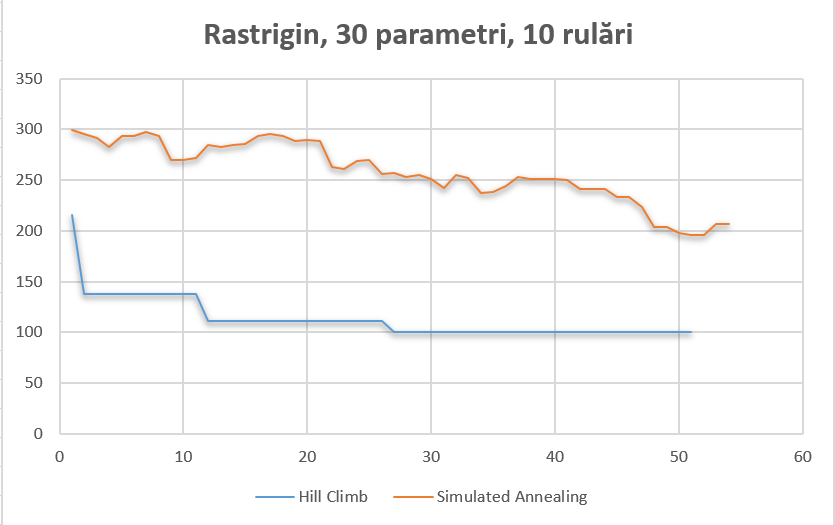
\includegraphics[width=\linewidth]{Grafic.png}
\end{figure}

\end{document}